\section{Navrh}
V tejto časti sa budeme zaoberať návrhom nášho systému riadenia dronov vrátane hardvérových a softvérových komponentov a ich vzájomnej interakcie. Cieľom je poskytnúť komplexný prehľad návrhu systému vrátane technických špecifikácií a funkcií, aby ostatní mohli systém pochopiť a replikovať. Budeme tiež diskutovať o rôznych konštrukčných úvahách, ktoré boli súčasťou vývoja systému, a o tom, ako sme ich riešili.

\subsection{Výber dronu}
Po preskúmaní funkcií možných programovateľných dronov je najlepším zariadením kvadrokoptér Tello, ktorú vyvinula spoločnosť Ryze, ale podporuje ju spoločnosť DJI. Dron Tello je malý quadcopter určený na lietanie v interiéri, ktorý má procesor Intel. Má rozmery len 98 x 92,5 x 41 mm a váži len 87 gramov, čo uľahčuje jeho prepravu a manévrovanie v stiesnených priestoroch. Dron je vybavený 5 MP kamerou, ktorá dokáže zachytiť video s rozlíšením 720p pri 30 snímkach za sekundu, takže je vhodný na základné fotografovanie a videografiu. Má tiež optický snímač toku smerujúci nadol a infračervený snímač vzdialenosti, ktoré mu pomáhajú udržiavať stabilný let v interiéri.

\begin{figure}[ht!]
    \centering
    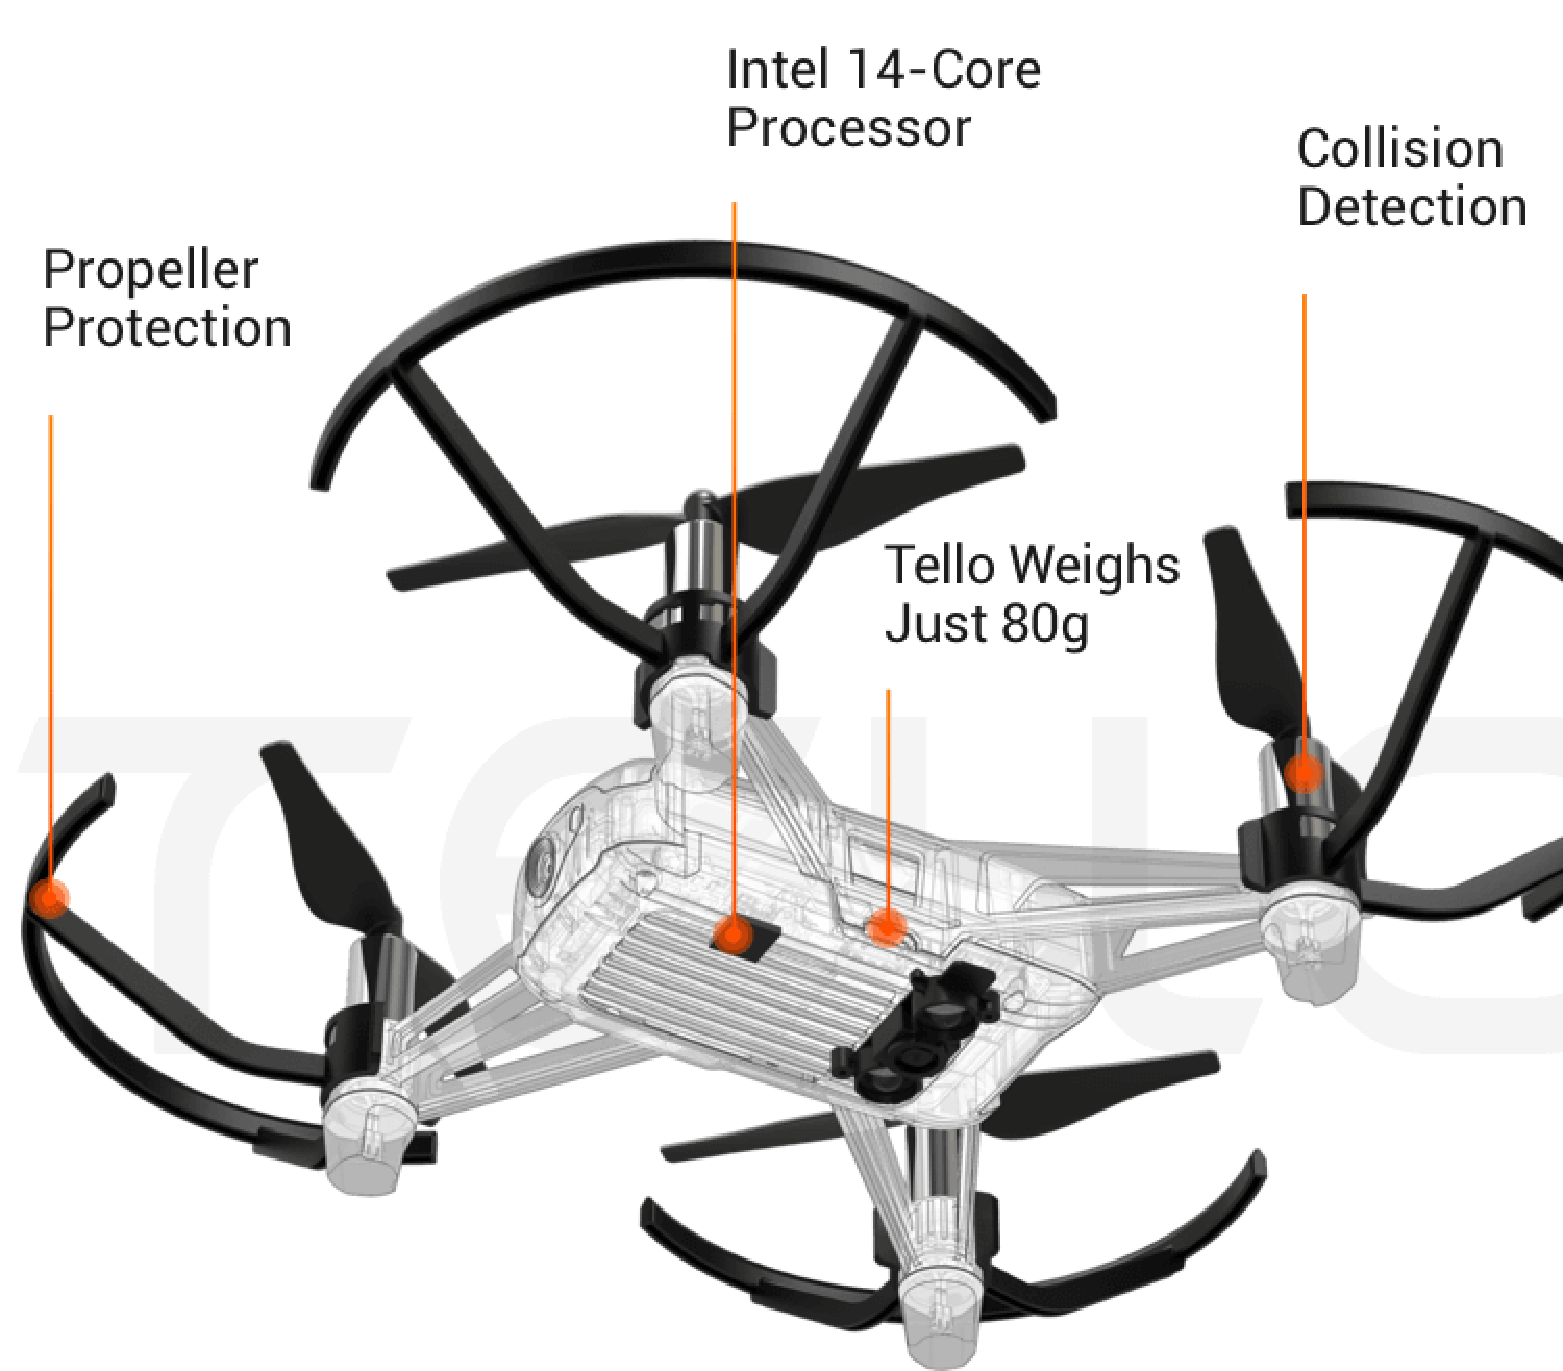
\includegraphics[width=.40\textwidth,angle=0]{figure 3-1.pdf}
    \caption{Dron DJI Tello a jeho komponenty.}
    \captionsetup{font=footnotesize, justification=centering, skip=5pt}
    \caption*{(Zdroj: www.ryzerobotics.com)}
    \label{o:3-1}
\end{figure} 

Dron Tello možno naprogramovať pomocou rôznych softvérových vývojových súprav (SDK). Jedným z populárnych SDK na programovanie dronu Tello je DJI Tello SDK, ktorý poskytuje súbor API na ovládanie letu, kamery a ďalších funkcií dronu. Súbor Tello SDK je k dispozícii pre viaceré programovacie jazyky vrátane jazykov Python, Java a Swift, vďaka čomu je prístupný vývojárom s rôznym vzdelaním a úrovňou zručností \citep{TelloSDK}.

Okrem DJI Tello SDK je k dispozícii aj niekoľko SDK a knižníc tretích strán na programovanie dronu Tello vrátane knižnice TelloPy pre Python a knižnice Node.js Tello pre Node.js. Tieto knižnice poskytujú ďalšie funkcie na ovládanie dronu a spracovanie údajov z jeho senzorov a môžu byť užitočné pre pokročilejšie projekty .

Celkovo je dron Tello všestrannou a cenovo dostupnou možnosťou pre interiérové aplikácie dronov a jeho podpora viacerých programovacích jazykov a SDK ho sprístupňuje vývojárom s rôznym vzdelaním a úrovňou zručností. 

\subsection{Programovací jazyk a súbor nástrojov}
Systém je založený na webovej aplikácii vyvinutej pomocou React, ktorá umožňuje používateľom ovládať drony v reálnom čase. Webová aplikácia komunikuje s backendovým serverom vytvoreným pomocou Node.js, ktorý funguje ako sprostredkovateľ medzi používateľom a dronmi \citep{TelloSDK}.

Frontend webovej aplikácie je vytvorený pomocou React, populárnej JavaScriptovej knižnice na vytváranie používateľských rozhraní. React umožňuje vytvárať opakovane použiteľné komponenty používateľského rozhrania, ktoré možno ľahko spravovať a aktualizovať. Okrem React využíva frontend aj ďalšie webové technológie, ako sú HTML5 a CSS3 \citep{TelloSDK}.

Backendový server je vytvorený pomocou Node.js, populárneho prostredia na spúšťanie JavaScriptu. Node.js umožňuje vytvárať škálovateľné a vysoko výkonné sieťové aplikácie, preto je vhodnou voľbou na vybudovanie backendu systému. Backendový server komunikuje s frontendom prostredníctvom rozhraní RESTful API a spojení WebSocket.

\begin{figure}[ht!]
    \centering
    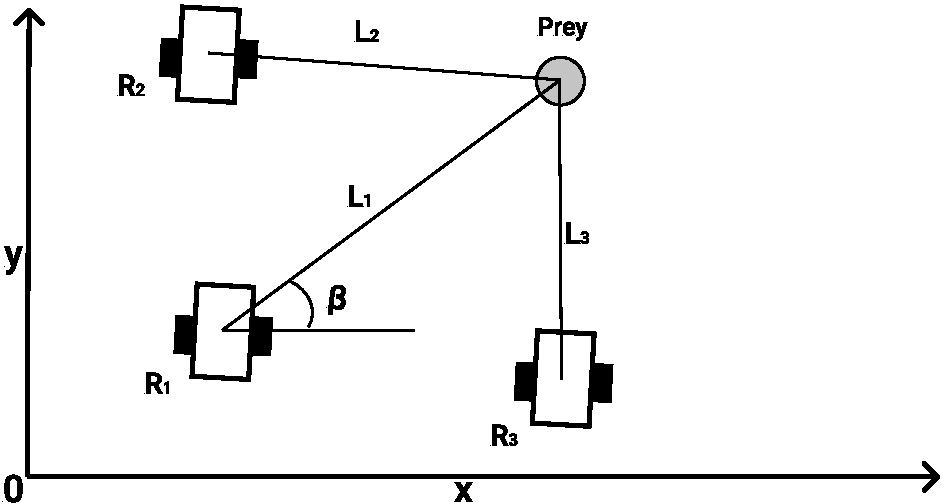
\includegraphics[width=.99\textwidth,angle=0]{figure 3-2.pdf}
    \caption{Schéma návrhu systému: Webová aplikácia vytvorená pomocou React komunikuje s backendovým serverom Node.js, ktorý posiela príkazy a prijíma telemetrické údaje z dronov pripojených k ASUS Tinkerboard.}
    \captionsetup{font=footnotesize, justification=centering, skip=5pt}
    \caption*{(Zdroj: vlastné spracovanie)}
    \label{o:3-2}
\end{figure}  

Na ovládanie dronov a prijímanie ich telemetrických údajov je backendový server pripojený k doske ASUS Tinker Board. Tinker Board je výkonný jednodoskový počítač, na ktorom beží upravená verzia systému Linux. Na každej doske Tinker Board je pre každý dron spustený program v jazyku Python. Tieto programy v jazyku Python sú zodpovedné za prijímanie príkazov z backendového servera a ich odosielanie do dronov, ako aj za prijímanie telemetrických údajov z dronov a ich odosielanie späť na backendový server.

Nakoniec systém využíva aj značky Aruco na zisťovanie polohy a orientácie dronov, ktoré sa používajú na riadenie pohybu dronov. Detekcia a sledovanie značiek Aruco sa vykonáva pomocou populárnej knižnice počítačového videnia OpenCV. Systém je tiež vybavený kamerou namontovanou na každom drone, ktorá zachytáva živý videozáznam, ktorý sa v reálnom čase prenáša späť do webovej aplikácie pomocou WebSocketov.
\subsection{Ako ovládať dron tello}
V dokumentácii poskytnutej výrobcom je podrobne opísané, ako ovládať dron pomocou programu Python. [19] Po pripojení k vlastnej sieti wifi dronu je potrebné otvoriť spojenie UDP na ovládanie dronu prostredníctvom adresy 192.168.10.1 a portu 8889. Pred spustením ovládania je vždy potrebné poslať dronu príkaz "command", ktorý sa prepne do stavu, v ktorom čaká na príkazy \citep{TelloSDK}. 
Z dronu je tiež možné čítať stav letového ovládača, ktorý využíva aj firmvér zariadenia, otvorením servera 0.0.0.0 na porte 8890. Ten nebol súčasťou vyššie uvedenej knižnice GitHub, preto sme ho do programu pridali. Otvorili sme nové spojenie so soketom UDP so spomínaným serverom a údajmi na porte bežiacim v samostatnom vlákne, podobne ako pri prijímaní odpovedí z kontroly dronu na pozadí. 

\begin{mypython}[caption={ukazuje obsluhu vlákna obsiahnutú v jazyku Python },label=SO-test]
    # Run Tello command responses UDP receiver on background
    client_socket = socket.socket(socket.AF_INET,socket.SOCK_DGRAM)
    response_receiver_thread = Thread(target=Tello.udp_response_receiver)
    response_receiver_thread.daemon = True
    response_receiver_thread.start()

    # Run state UDP receiver on background
    state_receiver_thread = Thread(target=Tello.udp_state_receiver)
    state_receiver_thread.daemon = True
    state_receiver_thread.start()

    threads_initialized = True
\end{mypython} 

  

Threading library, ktorý možno priradiť konkrétnej funkcii, 
ktorá bude bežať na vlákne oddelenom od hlavného programu. 
Vlákno, ktoré číta stav, ukazuje na funkciu get$_-$read$_-$state()
triedy Tello a spúšťa ju v samostatnom vlákne, takže beží na pozadí. Mali by ste zapnúť voľbu daemon = True, aby sa 
vlákno spúšťalo ako daemon, t. j. ak sa ukončí program vyššej úrovne, ukončí sa aj vlákno daemon. Ak táto možnosť nie 
je zapnutá, budete musieť ukončenia vlákien riešiť samostatne \citep{TelloSDK}.

Stavy vysiela dron na spomínanom serveri, ich čítanie nebude spomaľovať čítanie obrazu z kamery dronu, pretože dron bude vysielať reťazec stavov po vstupe do príkazového režimu, aj keď ho nebudeme čítať. V oficiálnej dokumentácii je uvedený formát, v ktorom dron vysiela stavy svojich senzorov. Vysiela jeden súvislý, stredníkmi ohraničený textový súbor ASCII cez bezdrôtové spojenie UDP na prijímajúci server v nasledujúcom formáte: \pyth{"pitch:%d;roll:%d;yaw:%d;vgx:%d;vgy:%d;vgz:%d;templ:%d;temph:%d;tof:%d;h:%d;bat:%d; baro:%.2f;time:%d;agx:%.2f;agy:%.2f;agz:%.2f;\r\n"}
Kde sú uvedené hodnoty jednotlivých stavov (interpretácia súradníc je uvedená na obrázku 8):
\begin{itemize}
\item \textbf{pitch, roll, yaw}: vlastná rotácia dronu okolo osí x, y a z, meraná ako celý uhol, kladný v smere hodinových ručičiek, podľa pravidla ľavej ruky;
\item \textbf{vgx, vgy, vgz}: rýchlosť dronu nastavená v smeroch x, y, z v cm/s (nie sú to skutočné merateľné hodnoty rýchlosti, ale hodnota priradená k rýchlosti dronu, ktorá sa mení počas riadenia);
\item \textbf{temp}: najnižšia teplota v C°; 
\item \textbf{temph}: najvyššia teplota v C° 
\item \textbf{tof}: výška kamery času letu v cm v spodnej časti dronu; 
\item \textbf{h}: výška v cm; 
\item \textbf{bat}: zostávajúca kapacita batérie dronu v celých percentách; 
\item \textbf{baro}: hodnota výšky na základe nainštalovaného barometra v cm; 
\item \textbf{time}: čas zapnutia motorov (čas letu) v sekundách; 
\item \textbf{agx, brain, agz}: zrýchlenie dronu v smere x, y, z zo snímača zrýchlenia interpretované v 0,001 g, kde g je gravitačné zrýchlenie. 
\end{itemize}

Toto sa dá rozdeliť na pole pozdĺž stredníkov pomocou funkcie Python string.split("; ") a potom sa hodnoty za dvojbodkou v poli prevedú na číselný typ v príslušnom formáte. Na číslo sa prevedú len požadované hodnoty a potom sa hodnoty načítajú do zoznamu, ktorý sa odovzdá do riadku. V Pythone je v rámci obsluhy vlákien len typ Queue, schopný zabezpečiť bezpečnu komunikáciu medzi vláknami; ak sa nepoužíva na výmenu údajov medzi vláknami v programe, program môže zamrznúť. 
\begin{mypython}[caption={Funkcia na čítanie stavov dronov },label=CL-2]
def get_read_state(self): 
    while True: 
        time.sleep(1/25) 
        try: 
            state_temp, _ = self.stateSocket.recvfrom(1024) 
            self.state = state_temp.decode('ASCII'). split(";") 
            pitch = -int(self.state[0][self.state[0].index(":")+1:]) 
            roll = -int(self.state[1][self.state[1].index(":")+1:]) 
            yaw = -int(self.state[2][self.state[2].index(":")+1:]) 
            tof = int(self.state[10][self.state[8].index(":")+1:]) 
            bat = int(self.state[10][self.state[10].index(":")+1:]) 
            self.data_queue.put([pitch, roll, yaw, tof, bat]) 
        except Exception as e: 
            self.LOGGER.error(e) 
\end{mypython} 
Počas riadenia máte tiež možnosť čítať stav tak, že pošlete do vlákna dotaz ako príkaz, na ktorý odpovie prostredníctvom spojenia UDP. Tieto dotazové slová poskytujú rovnaké stavy senzorov ako čítanie stavu (napr. : "akcelerácia?", "rýchlosť?", "batéria?", "tof?" ...). Zvažovalo sa aj použitie tejto funkcie, ale testy ukázali, že táto metóda poskytuje menej spoľahlivé výsledky. Táto komunikácia, na rozdiel od čítania stavu, spomaľuje a preťažuje ostatné funkcie dronu, pretože na reakciu na ne musí zabezpečiť samostatnú procesorovú kôru. Keďže teda nemôžeme získať spoľahlivé rezultáty ani s obsluhou vlákien, táto funkcia nie je pre naše účely užitočná. 

Obraz z kamery, ktorý je pre túto úlohu nevyhnutný, sa tiež vysiela cez UDP, pričom sa otvorí server 0.0.0.0 cez port 11111 \citep{Virbora2022}. Keďže veľkosť zakódovaných údajov obrazu je väčšia ako maximálna veľkosť užitočného zaťaženia prenosu UDP, obrazové údaje dron prenáša v blokoch po 1460 bajtov, z ktorých posledný blok je menší ako 1460 bajtov. Vysielaný obraz je možné po prijatí zobraziť pomocou balíka OpenCV. Balíky kodekov ffmpeg a libh264decoder uvedené v oficiálnej dokumentácii DJI-SDK preto v tomto prípade nie sú potrebné, testovanie programu prebieha pod operačným systémom MacOS \citep{Virbora2022}. 
Ovládacie inštrukcie SDK možno rozdeliť do troch skupín: 
\begin{enumerate}
\item inštrukcie na riadenie 
\begin{enumerate}
    \item vrátenie 'ok', ak sú splnené 
    \item "error" alebo chybové hlásenie, ak nie je 
\end{enumerate}
\item inštrukcie na čítanie 
\begin{enumerate}
    \item vráti hodnotu požadovaného parametra
\end{enumerate}
\item ovládanie nastavením parametrov 
\begin{enumerate}
    \item vrátenie 'ok', ak sú splnené 
    \item 'error' alebo chybové hlásenie, ak nie je 
\end{enumerate}
\end{enumerate}



Dronovi sa pošle príkaz "\pyth{takeoff}" (vzlet), vzlietne, pristane na príkaz "\pyth{land}" (pristátie), príkazy "\pyth{streamon}" (zapnutie) a "\pyth{streamoff}" (vypnutie) na prepnutie streamovania videa. Samotný dron je možné ovládať podľa smeru a súčasne príkazom "\pyth{go x y z speed}" (Obrázok 3-3). V tomto prípade sa dron bude pohybovať zadanou rýchlosťou vzhľadom na danú polohu v smere určenom tromi súradnicami. Presnosť tohto ovládania sa rovná rozmerom dronu, takže sa nemôže pohybovať o menej ako 20 centimetrov \citep{TelloSDK}. 

\begin{figure}[ht!]
    \centering
    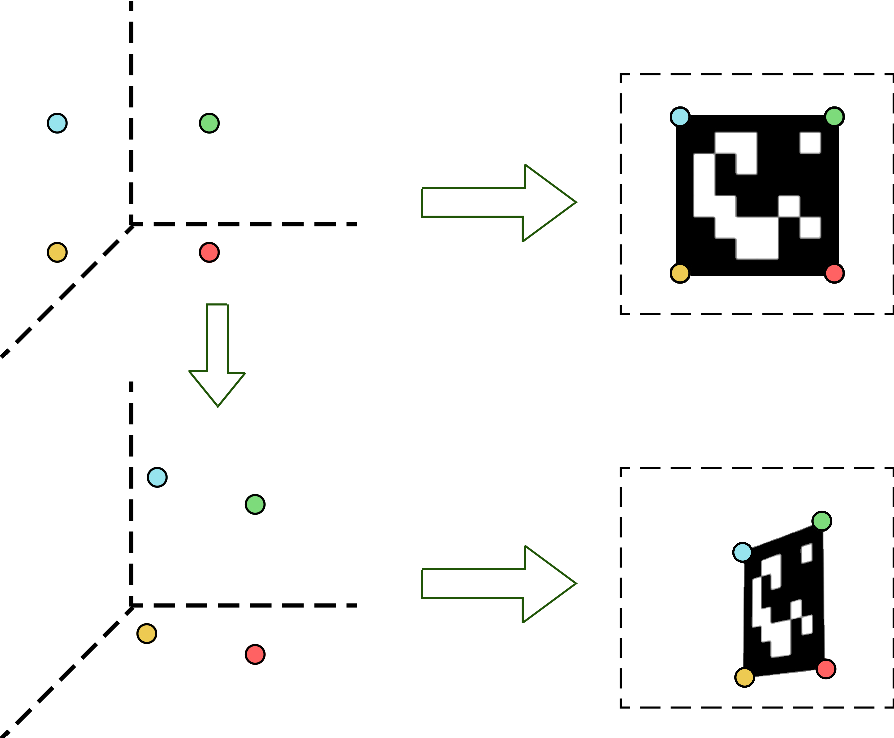
\includegraphics[width=.55\textwidth,angle=0]{figure 3-3.pdf}
    \caption{Smery definované pri ovládaní dronu pomocou SDK.}
    \captionsetup{font=footnotesize, justification=centering, skip=5pt}
    \caption*{(Zdroj: vlastné spracovanie)}
    \label{o:3-3}
\end{figure}  
Firmvér poskytuje aj možnosť ovládať dron v oblúku: zadaním ďalších dvoch bodov so súradnicami x, y, z vzhľadom na aktuálnu polohu dronu opíše nimi definovaný oblúk, ak je polomer oblúka v rozmedzí 0,5 až 10 metrov.

Pre túto úlohu je na základe testov s dronom najvhodnejším spôsobom riadenia tzv. RC riadenie, ktoré patrí do skupiny 3 spôsobov riadenia. Rýchlosti dronu v smeroch x, y, z a odklonu možno nastaviť príkazom "\pyth{rc x y z yaw}". S celočíselnými hodnotami od -100 do 100. (Rýchlosť yaw je tu tiež vyjadrená v súradnicovom systéme bal offset). Takto môžete dokonca vykresliť krivku odoslaním príkazov s danou frekvenciou za predpokladu, že hodnoty rýchlosti parametrickej krivky sú en- tované ako kontrola vzorkovaním s rovnakou frekvenciou. Pri tomto režime riadenia možno dosiahnuť menšie posuny ako pri už spomínaných príkazoch "go x y z speed". 
Do 2. skupiny inštrukcií patria inštrukcie, ktoré sa pýtajú na údaje zo senzorov. Napríklad aktuálne nastavenú rýchlosť, nabitie batérie, čas letu, nadmorskú výšku, zrýchlenie a uhlovú rýchlosť možno načítať z palubného ovládača dronu. Tieto sa nepoužívajú z dôvodu nespoľahlivej čitateľnosti, ktorá bola spomenutá vyššie \citep{TelloSDK}.

\subsection{Umiestnenie dronu}
Na zabezpečenie presného a spoľahlivého ovládania dronov je nevyhnutné optimálne umiestnenie dronov a značkovačov Aruco. Drony by mali byť umiestnené na otvorenom priestranstve s minimom prekážok a jasnou viditeľnosťou na značky. Značky by mali byť umiestnené tak, aby umožňovali maximálne pokrytie záujmovej oblasti a zároveň boli ľahko zistiteľné kamerou dronu.

Je tiež dôležité zabezpečiť, aby boli značky umiestnené v rovnakej výške a orientácii, čo uľahčí presnú detekciu a sledovanie. Do úvahy by sa mali brať aj akékoľvek zmeny svetelných podmienok, pretože môžu ovplyvniť detekciu a sledovanie značiek.

Okrem fyzického umiestnenia je tiež dôležité správne kalibrovať nastavenia dronu a kamery. To zahŕňa nastavenie parametrov, ako je rozlíšenie kamery, ohnisková vzdialenosť a korekcia skreslenia, aby sa zabezpečilo presné meranie a umiestnenie.

Dôkladným zvážením všetkých týchto faktorov možno umiestnenie dronu optimalizovať tak, aby sa dosiahol čo najlepší výkon a presnosť pre danú aplikáciu.

Údaje o zrýchlení by sa mohli použiť na určenie polohy, ale po odoslaní príkazu "zrýchlenie?" dáva čítanie veľmi nejasnú odpoveď. Dokonca aj po zmene časového limitu spojenia na požiadavku odosielanú s intervalom 0,1 sekundy nastaveného počas testov, stále dával zmysluplnú odpoveď po 0,5 sekundy, ale často len vyhadzoval chybu timeout. Takto boli prirodzene zašumené údaje akcelerometra načítané dokonca so značným vzorkovacím šumom. 

Druhou možnosťou je otvoriť server bežiaci v samostatnom vlákne, ktorý bude prijímať už spomínané stavové údaje. V tomto prípade dostávate údaje v jednom reťazci vrátane údajov akcelerometra a gyroskopu. Tieto údaje by bolo potrebné najprv prehnať cez ďalší filter \citep{7859621} alebo Kalmanov filter \citep{8839496} na odstránenie šumu zo senzorov. Dvojnásobnou integráciou hodnôt zrýchlenia možno získať posun dronu, ale integračná operácia zosilňuje šum, podlieha integračnej chybe a nedá sa korigovať v prípade absencie stabilných bodov polohy. Táto možnosť bola zavrhnutá z dôvodu akumulácie šumu pri integrácii. 

Preto sa vybrali značky ArUco, na základe ktorých možno merať relatívny posun kamery. Problémom pri nich je, že údaje o polohe možno získať len vtedy, keď je značka jasne viditeľná v obraze kamery. Tento problém sa však dá vyriešiť správnym označením testovacej plochy. Na umiestnenie značiek by sa mali použiť vhodné pravidlá, ktoré boli sformulované v časti 2.2.4, a tak možno určiť polohu kamery. 

\subsubsection{Používanie značkovačov aruco}
Funkcie potrebné na generovanie značiek ArUco nájdete v balíku prídavných modulov OpenCV-Contrib. Ich umiestnenie si vyžaduje kalibráciu kamery, ktorú možno vykonať aj pomocou kalibračného algoritmu v OpenCV na základe štúdie Z. Zhanga \citep{888718} odhadom parametrov kamery. 

Na kalibráciu potrebujete šachovnicu s dĺžkami strán, číslami riadkov a stĺpcov jej políčok. Na základe týchto údajov algoritmus vygeneruje teoretickú mapu vnútorných rohových bodov štvorcov a potom na základe vzoriek kamery vypočíta vnútorné a vonkajšie vlastnosti kamery v transformačných maticiach. Matica fotoaparátu obsahuje päť vnútorných vlastností fotoaparátu vrátane ohniskovej vzdialenosti, pomeru strán obrazového snímača a hlavného bodu dierkovej komory mod- elu. Získava sa aj matica skreslenia objektívu spojená s nelineárnymi vnútornými vlastnosťami, ktorú možno použiť na odstránenie súdkovitého a poduškovitého skreslenia na okrajoch obrazu. Vonkajšie (vonkajšie) vlastnosti kamery sú tiež opísané transformačnou maticou, ktorá realizuje prevod zo súradníc reálneho 3D priestoru na 3D súradnice kamery(Obrázok 3-5). Matica aplikuje homogénnu transformáciu: posun do stredu (počiatku) snímača kamery o vektor T a rotáciu o maticu rotácie R. 

\begin{figure}[ht!]
    \centering
    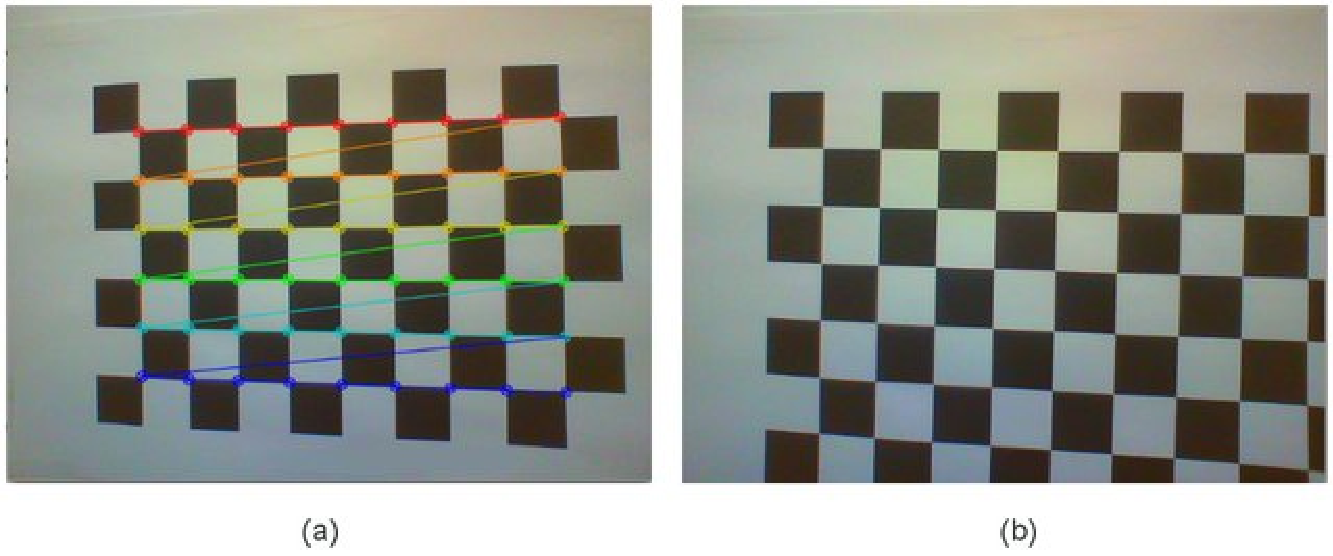
\includegraphics[width=.90\textwidth,angle=0]{figure 3-4.pdf}
    \caption{Tradičná kalibrácia pomocou vzoru šachovnice. a) Rutiny OpenCV dokážu odhaliť všetky rohy šachovnice. b) Rohy nemožno priradiť k príslušným bodom na vzore šachovnice, ak vzor nie je úplne zachytený.}
    \captionsetup{font=footnotesize, justification=centering, skip=5pt}
    \caption*{(Zdroj: vlastné spracovanie)}
    \label{o:3-4}
\end{figure}  

\begin{figure}[ht!]
    \centering
    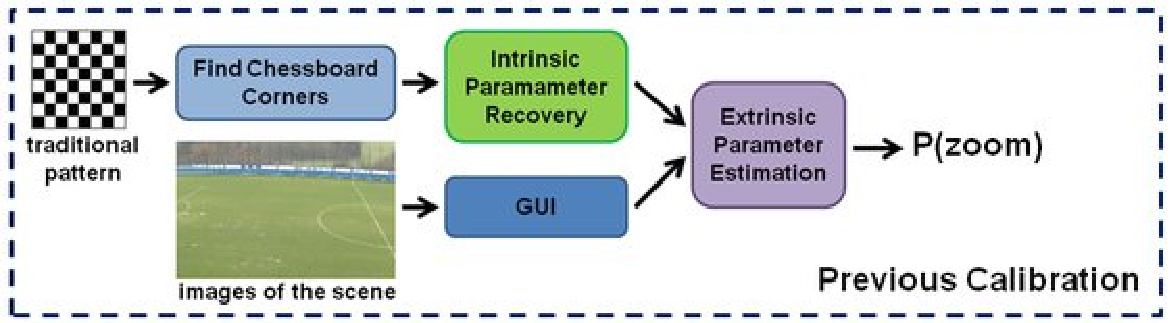
\includegraphics[width=.90\textwidth,angle=0]{figure 3-5.pdf}
    \caption{Schéma procesu kalibrácie.}
    \captionsetup{font=footnotesize, justification=centering, skip=5pt}
    \caption*{(Zdroj: vlastné spracovanie)}
    \label{o:3-5}
\end{figure}  

Teoreticky by na správnu kalibráciu mali stačiť dve vzorky, ale na dosiahnutie presnejších údajov pracujeme s 20 súbormi údajov. Fotografia na obrázku 3-4 bola zhotovená počas procesu kalibrácie. Výsledné matice sa ukladajú do súboru s názvom camcalib.npz a čítajú sa z neho, aby sa pred každým použitím nemusela kalibrovať zabudovaná kamera dronu. 

Jedným z najčastejších zdrojov chýb pri meraní kamerou je súdkovité skreslenie, ktoré možno odstrániť pomocou matice skreslenia získanej počas kalibrácie pomocou vstavanej funkcie OpenCV cv2.undistort(). Tým sa zníži efekt rybieho oka a do určitej miery sa zmenší zorné pole, ale získajú sa presnejšie hodnoty na okrajoch obrazu pre následné umiestnenie pomocou značiek ArUco.
\subsubsection{Pravidlá umiestňovania značiek}
Pri používaní značkovačov Aruco na určovanie polohy dronov je potrebné dodržiavať niekoľko dôležitých pravidiel, aby sa zabezpečili presné a spoľahlivé výsledky. Tu je niekoľko pokynov pre umiestnenie značiek \citep{Marut2019}:
\begin{enumerate}

\item \textbf{Dostatočný počet značiek}: Na presné sledovanie polohy a orientácie dronu je dôležité použiť dostatočný počet značiek. To pomôže zabezpečiť, aby boli značky vždy viditeľné z pohľadu dronu, aj keď sa dron rýchlo pohybuje;

\item \textbf{Značky umiestnite do mriežky}: Umiestnenie značiek do pravidelnej mriežky pomôže zabezpečiť ich rovnomerné rozloženie a viditeľnosť z viacerých uhlov. To môže tiež pomôcť znížiť pravdepodobnosť zákrytov alebo iných problémov, ktoré by mohli narušiť sledovanie;

\item \textbf{Vyber veľkosti značiek}: Veľkosť použitých značiek bude závisieť od vzdialenosti, z ktorej sa na ne bude pozerať. Napríklad, ak bude dron lietať relatívne blízko značiek, môžete použiť menšie značky. Ak však bude dron vo väčšej vzdialenosti, možno budete musieť použiť väčšie značky, aby ste zabezpečili viditeľnosť;

\item \textbf{Reflexný alebo priehľadný povrch}: Reflexné alebo priehľadné povrchy môžu narušiť detekciu značiek tým, že spôsobujú odrazy alebo lomy, ktoré skresľujú vzhľad značky. Aby ste sa vyhli tomuto problému, vyberte si miesto na umiestnenie značky, ktoré je bez reflexných alebo priehľadných povrchov;

\item V zornom poli dronu musí byť vždy prítomný aspoň jedna značka, aby sa zabezpečilo, že dron môže nepretržite sledovať svoju polohu a orientáciu;

\item Keď sa značky časom zistia a stratia, systém použije polohu a orientáciu predchádzajúceho značky na odhad aktuálnej polohy a trajektórie dronu, kým sa nezistí novu značku.
\end{enumerate}


\subsection{Prvé testy polohovania pomocou značiek}
Na testovanie sa použili štyri značky 7x7 ArUco s dĺžkou strany 0,0957 m z knižnice DICT-7x7-100. K dispozícii sú aj značky s plochami 4x4, 5x5 a 6x6, ale vyššie rozlíšenie knižnice 7x7 umožňuje presnejšie určovanie polohy. V každej knižnici je k dispozícii až 1024 rôznych značiek, čo by malo stačiť na poskytnutie informácií potrebných na riadenie dronu.

Odporúča sa používať viac ako jedna značka, pretože systém dokáže spriemerovať z viacerých hodnôt, takže spriemerovaním možno získať presnejšie výsledky, jednoducho odfiltrovaním akýchkoľvek odľahlých hodnôt. Okrem toho, ak je v zornom poli dronu niekoľko značiek, je menší problém, ak sa jedna z nich stratí, pretože stále môže čítať hodnoty z ostatných. V prvom experimente boli značky umiestnené kolmo na kameru dronu, vertikálne k stene, ako je znázornené na fotografii na obrázku 10. Cieľom tohto testu bolo zistiť, ako dobre dokáže softvér ukladať údaje, ktoré sa približujú realite.

Súbor bodov vľavo na obrázku 11 ukazuje, že súbor meracích bodov bol úspešne sledovaný hneď po opísaní štvorca dronom a dokonca aj po zakreslení jednej z jeho uhlopriečok, a vpravo ukazuje, že aj zmena výšky bola pomocou značiek zistená s vynikajúcou presnosťou. Priesečník čiernych osí je počiatok pohybu dronu. Body na obrázku vyznačené červenou farbou sú skutočné hodnoty a zelená krivka je B-spline krivka prispôsobená bodu nastavenému funkciou splprep() v podadresári interpolate balíka Scipy dostupného v programovacom jazyku Python. Parameter spresnenia funkcie bol po niekoľkých experimentoch na základe dokumentácie \citep{scipy-docs} zvolený na hodnotu s=0,1, čo al- ready dostatočne aproximuje množinu bodov odfiltrovaním zašumených bodov. Nakoniec sme vo finálnej verzii programu použili na filtrovanie dátových bodov Kalmanov filter namiesto metódy B-spline interpolácie, pričom sme mysleli na budúcu implementáciu v reálnom čase a adaptívnejšie správanie Kalmanovho filtra. 

Jediná korekcia, ktorú bolo potrebné aplikovať na experimentálnu sadu bodov, bolo negatívne otočenie bodov o 10,5° okolo osi x, inak by sa Z-koordináty bodov zväčšili, keď by sa približovali k značkám, a to aj pri konštantnej výške. Je to spôsobené uhlom kamery od vodnej hladiny, pričom pri priblížení k markerom sa zistila vyššia poloha. (Toto bude neskôr zbytočné kvôli korekcii uhlového natočenia značiek.)

V tomto nastavení bude dron poskytovať skutočné hodnoty posunutia len vtedy, ak je rovina kamery (okrem uhla poklesu) rovnobežná s rovinou značiek. Ak sa poloha od tejto odchýli, dron bude udávať nesprávne hodnoty. Hodnoty posunutia sa musia odhadnúť s prihliadnutím na uhly natočenia, inak nemôžeme previesť hodnoty vektorov translácie značiek ArUco do súradnicového systému prvej videnej značky, ktorý chceme použiť ako globálny súradnicový systém.  Hodnoty vektorov zadané funkciou cv2.aruco.estimatePoseSingleMarkers() balíka OpenCV sú zadané v súradnicovom systéme kamery, ktoré je potom potrebné previesť do súradnicového systému značiek. 

\subsubsection{Vyhodnotenie testu a očakávania od systému}
Na základe prvých testov sa oplatí ďalej skúmať túto možnosť určovania polohy, pretože dokáže vypočítať polohu dronu v reálnom čase s relatívne malým počtom transformácií. Bohužiaľ, nemôžeme využiť grafickú akceleráciu balíka CUDA, ktorú poskytuje spoločnosť Nvidia, pretože funkcie balíka OpenCV-Python neboli všetky pridané do knižnice cv2.cuda v jazyku Python. Spomalí to spracovanie obrazu, ale aj tak spôsobí väčšie oneskorenie operácie kvôli 1,5...2 sekundovému oneskoreniu kamerového obrazu prenášaného dronom. 

Očakáva sa, že chyba merania metódy bude približne 0,05 m pri zväčšenej veľkosti značiek a vhodnom počte značiek. V dôsledku konverzií medzi súradnicovými systémami značiek však môžeme očakávať aj chybu driftu, ktorá sa zvyšuje so vzdialenosťou od značky reprezentujúceho globálnu súradnicu v dôsledku nepresnosti transformácií medzi súradnicovými systémami.

\subsection{Princíp, spresnenie a robustnosť polohovania}
Počas vývojovej a testovacej fázy kamerového programu sme namiesto palubnej kamery dronu Tello použili webovú kameru. Dôvodom bola predovšetkým obmedzená životnosť batérie dronu, ktorá by sťažila testovanie a zdokonaľovanie programu na dlhší čas. Namiesto toho sme použili webovú kameru namontovanú na stabilnej platforme, ktorá simulovala pohľad kamery dronu, a testovali sme výkon programu v rôznych svetelných podmienkach, vzdialenostiach a orientáciách. Keď sme boli s výkonom programu spokojní, preniesli sme ho do dronu Tello a podľa potreby sme vykonali drobné úpravy.
Program bol napísaný s použitím funkcií poskytovaných v balíku OpenCV ArUco, napríklad:
\begin{enumerate}
\item \textbf{Detekcia a rozpoznávanie značiek}: Na detekciu a rozpoznanie značiek Aruco vo videokanáli dronu používame funkciu cv2.detectMarkers(). Táto funkcia prijíma obraz, slovník Aruco a parametre na detekciu a vracia zistené značky a ich príslušné ID;
\item \textbf{Transformácie medzi súradnicovými systémami značky a kamery}: Po zistení a rozpoznaní značiek musíme transformovať ich polohu v obraze (v pixelových súradniciach) na ich polohu v súradnicovom systéme kamery (v milimetroch). Toto sa vykoná pomocou funkcie cv2.aruco.estimatePoseSingleMarkers(), ktorá prijme detekované značky, veľkosť značiek, maticu kamery a koeficienty skreslenia a vráti vektory rotácie a translácie, ktoré predstavujú polohu každej značky v súradnicovom systéme kamery;
\item \textbf{Spresnenie pozícií značiek}: Keďže zistené polohy značiek nie sú vždy presné, musíme ich spresniť pomocou subpixelovej presnosti. To sa vykonáva pomocou funkcie cv2.cornerSubPix(), ktorá prijíma obraz, zistené rohy značky a parametre pre subpixelové spresnenie a vracia spresnené rohové pozície;
\item \textbf{Robustnosť polohovania}: Aby sme zabezpečili robustnosť a presnosť polohy dronu, používame v obraze viacero značiek a vykonávame priemerovanie ich polôh. To pomáha znížiť vplyv šumu a chýb pri detekcii a rozpoznávaní značiek;
\item \textbf{Transformácia perspektívy a bodu (PnP)}: Funkcia cv2.aruco.solvePnP() sa používa na odhad pózy (polohy a orientácie) značky v 3D priestore. Táto funkcia prijíma ako vstup 2D súradnice značky na obrázku, 3D súradnice značky v reálnom svete a maticu kamery, ktorá obsahuje vlastné parametre kamery (ohniskovú vzdialenosť, hlavný bod atď.) \citep{9549863}.
\end{enumerate}

\begin{figure}[ht!]
    \centering
    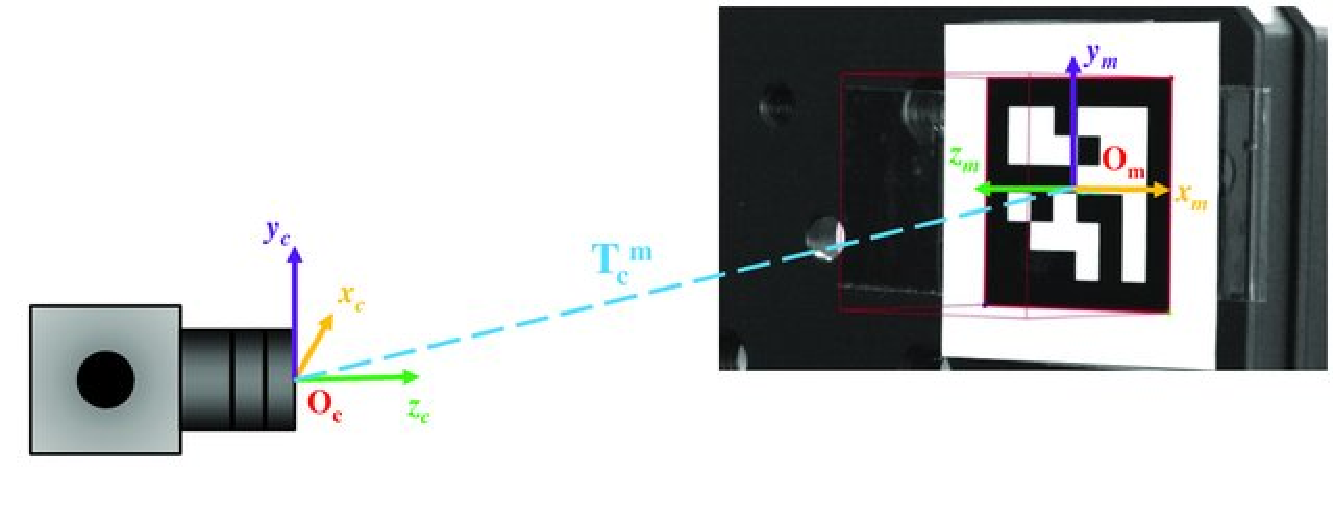
\includegraphics[width=.90\textwidth,angle=0]{figure 3-6.pdf}
    \caption{Súradnicový systém kamery a značky interpretovaný programom OpenCV.}
    \captionsetup{font=footnotesize, justification=centering, skip=5pt}
    \caption*{(Zdroj: Popescu, Dragos. (2018). Automatic rough alignment for key components in laser driven experiments using fiducial markers. Journal of Physics: Conference Series. 1079. 012013. 10.1088/1742-6596/1079/1/012013.)}
    \label{o:3-6}
\end{figure}  
% Popescu, Dragos & Cernaianu, Mihail & Dumitrache, I.. (2018). Automatic rough alignment for key components in laser driven experiments using fiducial markers. Journal of Physics: Conference Series. 1079. 012013. 10.1088/1742-6596/1079/1/012013. 

\subsubsection{Perspektívna projekcia, transformácia pnp}
Perspektívna projekcia je matematická metóda, ktorá sa používa na transformáciu 3D objektov na 2D obrazovú rovinu. Tento vzťah sa nazýva perspektívna projekcia a je založený na princípe podobnosti trojuholníkov. Matematicky môžeme tento proces zapísať ako \citep{9549863}:
\begin{equation}
    \begin{pmatrix} u \\ v \\ 1 \end{pmatrix} =
    \begin{bmatrix}
        f_x & 0 & c_x \\
        0 & f_y & c_y \\
        0 & 0 & 1
    \end{bmatrix}
    \begin{bmatrix}
        r_{11} & r_{12} & r_{13} & t_1 \\
        r_{21} & r_{22} & r_{23} & t_2 \\
        r_{31} & r_{32} & r_{33} & t_3 \\
        0 & 0 & 0 & 1
    \end{bmatrix}
    \begin{bmatrix}
        X \\ 
        Y \\
        Z \\
        1
    \end{bmatrix}
\end{equation}
kde $u$ a $v$ sú pixely v 2D obrazovke, $(X, Y, Z)$ sú súradnice bodu v 3D priestore, $fx$ a $fy$ predstavujú ohniskovú vzdialenosť kamery v osiach $x$ a $y$ v pixely, $cx$ a $cy$ predstavujú súradnice stredu obrazovky v pixely, $r_{11}$ až $r_{33}$ sú prvky rotácie a $t_1$ až $t_3$ predstavujú posun kamery v priestore.

Tento proces zahŕňa vytvorenie modelu kamery, ktorý definuje polohu a orientáciu virtuálnej kamery v 3D priestore. Tento model kamery sa potom použije na premietnutie 3D súradníc objektu do 2D roviny.

Na výpočet transformácie medzi 3D svetovými súradnicami objektu a jeho 2D obrazovými súradnicami sa používa algoritmus PnP (Perspective-n-Point). Túto transformáciu možno použiť na určenie polohy a orientácie objektu v 3D priestore vzhľadom na kameru.

Algoritmus PnP vyžaduje nasledujúce vstupy:
\begin{enumerate}
\item Súbor 3D bodov objektu vyjadrených v súradnicovom systéme vzhľadom na kameru;
\item Súbor 2D obrazových bodov, ktoré zodpovedajú projekcii 3D bodov objektu na 2D obrazovú rovinu;
\item Vlastná matica kamery, ktorá opisuje vnútorné parametre kamery, ako je ohnisková vzdialenosť a hlavný bod;
\item Voliteľne vonkajšia matica kamery, ktorá opisuje polohu a orientáciu kamery v 3D priestore;
\item Algoritmus PnP vypočíta rotáciu a transláciu objektu vzhľadom na kameru pomocou nelineárnej optimalizačnej metódy. Algoritmus minimalizuje chybu reprojekcie, čo je rozdiel medzi projektovanými 3D bodmi a zodpovedajúcimi 2D obrazovými bodmi.
\end{enumerate}

Algoritmus PnP možno riešiť rôznymi metódami vrátane metódy priamej lineárnej transformácie (DLT) a Levenberg-Marquardtovho algoritmu. Metóda DLT zahŕňa riešenie lineárnej sústavy rovníc, zatiaľ čo Levenberg-Marquardtov algoritmus je nelineárna optimalizačná metóda.

Algoritmus PnP je základným nástrojom počítačového videnia a používa sa v mnohých aplikáciách vrátane sledovania objektov, rozšírenej reality a lokalizácie robotov.

Algoritmus PnP je implementovaný vo funkcii OpenCV cv2.solvePnP(), ktorá prijíma vyššie opísané vstupy a vracia vektory rotácie a translácie objektu vzhľadom na kameru. Tieto vektory možno použiť na transformáciu súradníc objektu do súradnicového systému kamery alebo naopak pomocou jednoduchých maticových operácií \citep{opencv_calib3d}.

Vzorec pre transformáciu PnP je nasledujúci:
\begin{equation}
    rvec, tvec = cv2.solvePnP(objectPoints, imagePoints, cameraMatrix, distCoeffs)
\end{equation}
kde:
\begin{enumerate}
\item $\text{objectPoints}$ je pole 3D bodov v súradnicovom systéme objektu;
\item $\text{imagePoints}$ je pole zodpovedajúcich 2D obrazových bodov;
\item $\text{cameraMatrix}$ je vlastná matica kamery;
\item $\text{distCoeffs}$ sú koeficienty skreslenia kamery;
\item $rvec$ je vektor natočenia objektu vzhľadom na kameru;
\item $tvec$ je vektor translácie objektu vzhľadom na kameru.
\end{enumerate}

Vektor rotácie rvec možno previesť na maticu rotácie pomocou funkcie cv2.Rodrigues(). Translačný vektor tvec je vyjadrený v súradnicovom systéme kamery a možno ho použiť na transformáciu súradníc objektu do súradnicového systému kamery pomocou jednoduchej maticovej operácie \citep{opencv_calib3d}:
\begin{equation}
    \textbf{objectPoints}{\textbf{cam}} = \textbf{R} \cdot \textbf{objectPoints}^{\top} + \textbf{t}{\textbf{vec}}
    \end{equation}
Kde $\textbf{objectPoints}{\textbf{cam}}$ je transformované pole 3D bodov objektu v súradnicovom systéme kamery, $\textbf{R}$ je matica rotácie, $\textbf{objectPoints}$ je pole 3D bodov objektu v súradnicovom systéme objektu, $\textbf{t}{\textbf{vec}}$ je vektor translácie objektu vzhľadom na kameru a $\cdot$ predstavuje násobenie matíc.

\subsubsection{Konvencie merania}
Pri riešení problémov počítačového videnia je dôležité stanoviť súbor konvencií merania. Tieto konvencie špecifikujú súradnicový systém používaný na reprezentáciu polôh a orientácií objektov v 3D priestore, ako aj jednotky používané na ich meranie. V tejto časti opíšeme konvencie používané v počítačovom videní, ktoré sú založené na pravotočivom súradnicovom systéme.

\textbf{Pravotočivý súradnicový systém.} Pravotočivý súradnicový systém je najčastejšie používaným systémom v počítačovom videní. Je to trojrozmerný karteziánsky súradnicový systém, v ktorom kladné osi x, y a z smerujú doprava, nahor a k pozorovateľovi. Orientáciu súradnicového systému možno reprezentovať pomocou matice rotácie, ktorá transformuje body zo svetového súradnicového systému do súradnicového systému kamery.

\textbf{Jednotky merania.} Merné jednotky používané v počítačovom videní sú zvyčajne milimetre alebo metre. Tieto jednotky sa používajú na reprezentáciu vzdialeností, napríklad vzdialenosti medzi dvoma bodmi v 3D priestore alebo ohniskovej vzdialenosti kamery. Výber jednotiek závisí od rozsahu riešeného problému.

\textbf{Matica kamery.} Matica kamery je matica 3x4, ktorá predstavuje vnútorné a vonkajšie parametre kamery. Vnútorné parametre opisujú vlastnosti kamery, napríklad ohniskovú vzdialenosť a polohu hlavného bodu, zatiaľ čo vonkajšie parametre opisujú orientáciu a polohu kamery v 3D priestore. Maticu kamery možno zapísať ako:

\begin{equation}
\mathbf{P} = \begin{bmatrix}f_x & 0 & c_x & t_x \\ 0 & f_y & c_y & t_y \\ 0 & 0 & 1 & 0\end{bmatrix},
\end{equation}

kde $f_x$ a $f_y$ sú ohniskové vzdialenosti v smere x a y, $c_x$ a $c_y$ sú súradnice hlavného bodu v obraze a $t_x$ a $t_y$ sú translačné parametre, ktoré opisujú polohu kamery vo svetovom súradnicovom systéme.

\textbf{Projekčná matica.} Projekčná matica je matica 3x4, ktorá mapuje 3D body vo svetovom súradnicovom systéme na 2D body v súradnicovom systéme obrazu. Vypočíta sa ako súčin matice kamery a matice rotácie, ktorá transformuje body zo svetového súradnicového systému do súradnicového systému kamery:

\begin{equation}
\mathbf{P'} = \mathbf{P} \cdot [\mathbf{R} | \mathbf{t}],
\end{equation}
kde $\mathbf{R}$ je matica rotácie a $\mathbf{t}$ je vektor translácie, ktorý opisuje polohu kamery vo svetovom súradnicovom systéme.

\textbf{Homogénny súradnicový systém.} Homogénny súradnicový systém je matematický rámec, ktorý nám umožňuje reprezentovať body v 3D priestore ako 4D vektory. Je to užitočné, pretože nám to umožňuje vykonávať transformácie, ako je translácia a rotácia, pomocou násobenia matíc. 3D bod $\mathbf{X} = [X, Y, Z]$ vo svetovom súradnicovom systéme možno reprezentovať v homogénnych súradniciach ako $\mathbf{X}_h = [X, Y, Z, 1]$. Podobne bod $\mathbf{x} = [u, v]$ v súradnicovom systéme obrazu možno reprezentovať v homogénnych súradniciach ako $\mathbf{x}_h = [u, v, 1]$.

Keďže neexistuje všeobecná dohoda o konvencii pre Eulerove uhly, musíme definovať používanú konvenciu. V tomto prípade ukladáme uhly v už spomínanom poradí podľa záporných hodnôt získaných z dronu SDK. Tie sú totožné s konvenciou uhlov používanou pre lietadlá podľa letovej normy DIN 9300-2 (obrázok 3-6). Presnejšou definičnou skupinou pre konvenciu vybraných uhlov je vlastná konvencia Tait-Bryanových uhlov z-y'-x", známa aj ako námorné alebo Cardanove uhly \citep{DIN9300-2}.
\begin{figure}[ht!]
    \centering
    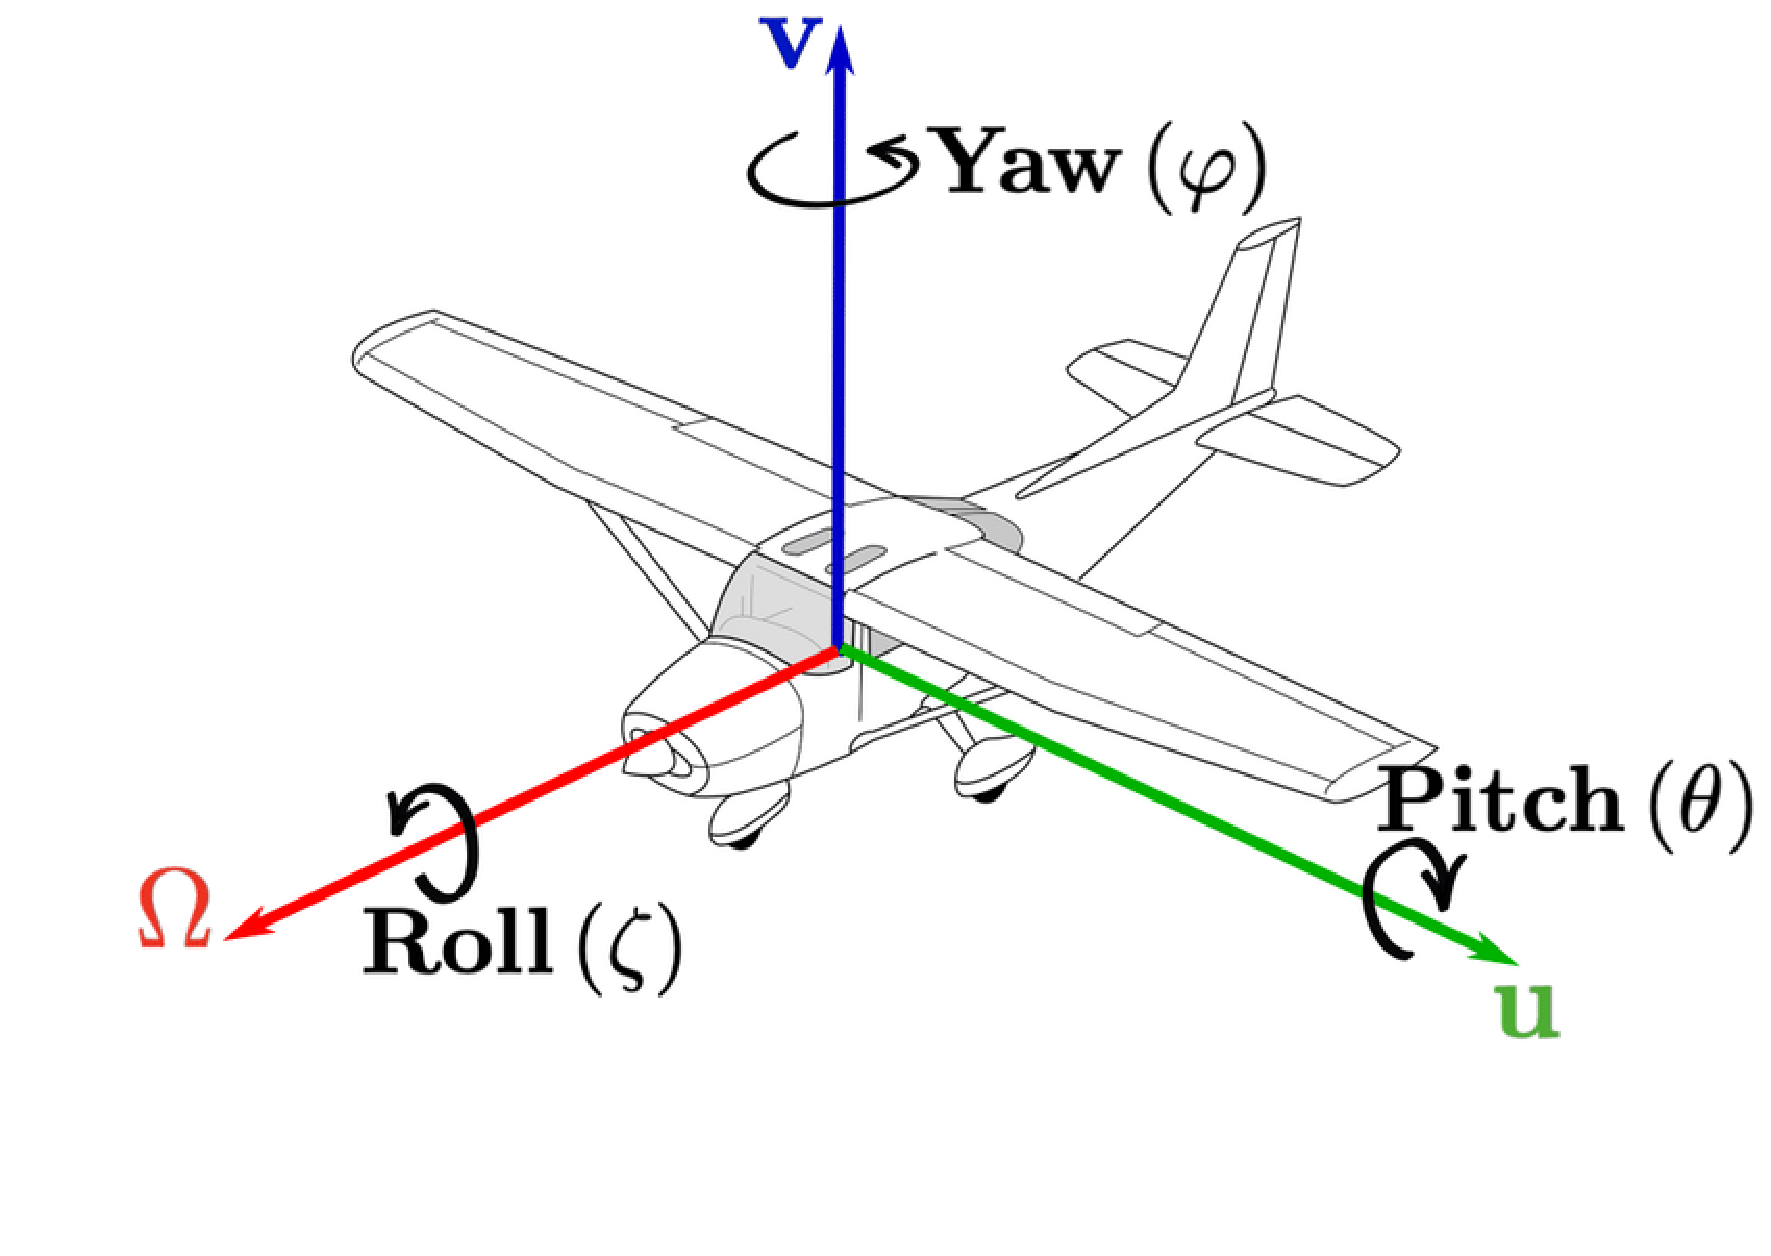
\includegraphics[width=.65\textwidth,angle=0]{figure 3-8.pdf}
    \caption{Hlavné nápravy lietadla podľa normy DIN 9300.}
    \captionsetup{font=footnotesize, justification=centering, skip=5pt}
    \caption*{(Zdroj: vlastné spracovanie)}
    \label{o:3-8} 
\end{figure} 

\subsubsection{Konvencie používané v opencv}
OpenCV používa špecifický súbor konvencií na reprezentáciu bodov, rotácií a translácií \citep{opencv_calib3d}. Tieto konvencie je dôležité pochopiť pri práci s knižnicou. Tu sú niektoré z hlavných konvencií používaných v OpenCV:

Body sú reprezentované ako súradnice (x, y) s počiatkom (0, 0) v ľavom hornom rohu obrazu.

Rotácie sú reprezentované pomocou Rodriguesovho rotačného vzorca, ktorý konvertuje 3D rotačný vektor na 3x3 rotačnú maticu. Vektor rotácie je definovaný ako (rx, ry, rz), kde rx, ry a rz predstavujú uhly rotácie okolo osí x, y a z.

Translácie sú reprezentované ako 3D vektory (tx, ty, tz).

Vlastné parametre kamery sú reprezentované pomocou nasledujúcej matice:
\begin{equation}
\begin{bmatrix}
f_x & 0 & c_x \\
0 & f_y & c_y \\
0 & 0 & 1
\end{bmatrix}
\end{equation}

kde fx a fy sú ohniskové vzdialenosti kamery v smere x a y a cx a cy sú súradnice hlavného bodu (bod, v ktorom optická os pretína rovinu obrazu).

Vonkajšie parametre kamery sú reprezentované pomocou matice 3x4, ktorá kombinuje rotáciu a transláciu:
\begin{equation}
\begin{bmatrix}
r_{11} & r_{12} & r_{13} & t_x \\
r_{21} & r_{22} & r_{23} & t_y \\
r_{31} & r_{32} & r_{33} & t_z
\end{bmatrix}
\end{equation}
kde ľavý horný stĺpec matice 3x3 predstavuje maticu rotácie a pravý stĺpec predstavuje vektor translácie.

Medzi hodnotami vrátenými funkciou estimatePoseSingleMarkers() sa vektor translácie interpretuje v metroch a vektor rotácie používa reprezentáciu osového uhla alebo Rodriguesovu reprezentáciu, čo je najkompaktnejšia forma uloženia matice rotácie. Funkcia Rodrigues() v OpenCV dokáže vypočítať maticu rotácie z vektorov rotácie zadaných ako riadkové vektory podľa rovnice (3.8.) a dokáže určiť aj jej inverziu, ak je vstupom matica rotácie.
\begin{figure}[ht!]
    \centering
    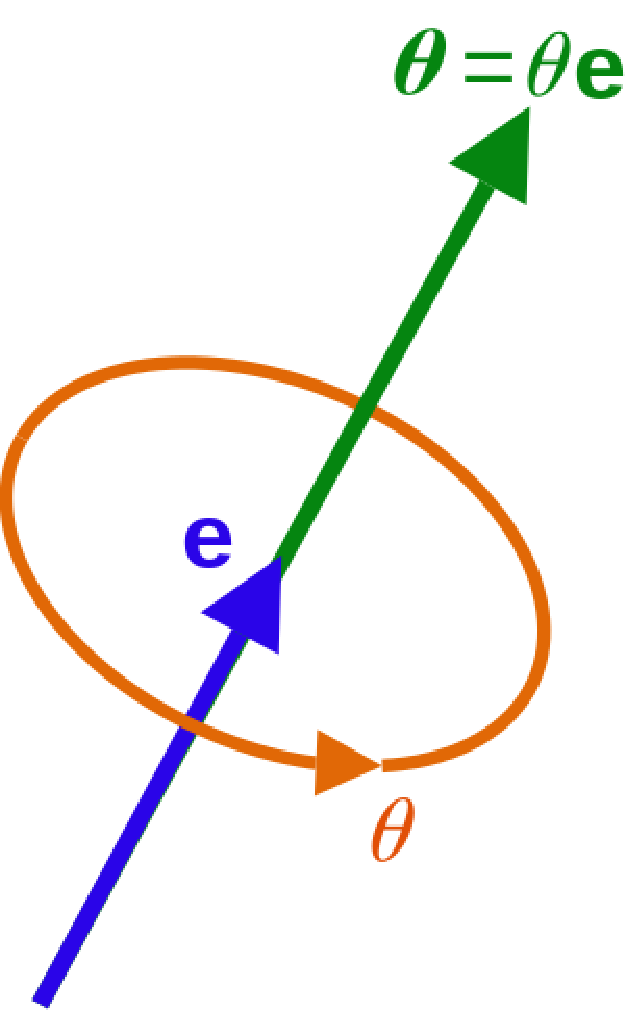
\includegraphics[width=.13\textwidth,angle=0]{figure 3-7.pdf}
    \caption{Interpretácia vektora natočenia Rodriguesovej osi a uhla.}
    \label{o:3-7} 
\end{figure}
% https://en.wikipedia.org/wiki/Axis%E2%80%93angle_representation

\subsubsection{Prevod polohy kamery do globálneho súradnicového systému}
Na prevod polohy kamery (ktorá sa nachádza v počiatku súradnicového systému kamery) do globálneho súradnicového systému musíme použiť vektory rotácie a translácie získané z funkcie solvePnP v OpenCV.

Vektor rotácie (rvec) udáva rotáciu súradnicového systému kamery vzhľadom na súradnicový systém značky a vektor translácie (tvec) udáva polohu značky v súradnicovom systéme kamery.

Na prevod polohy kamery do globálneho súradnicového systému musíme postupovať podľa týchto krokov:

\textbf{1. Vypočítame maticu rotácie R} z vektora rotácie rvec pomocou Rodriguesovho vzorca:
\begin{equation}
R = \begin{bmatrix}
\cos\theta + u_x^2(1-\cos\theta) & u_x u_y (1-\cos\theta) - u_z \sin\theta & u_x u_z (1-\cos\theta) + u_y \sin\theta \\
u_y u_x (1-\cos\theta) + u_z \sin\theta & \cos\theta + u_y^2(1-\cos\theta) & u_y u_z (1-\cos\theta) - u_x \sin\theta \\
u_z u_x (1-\cos\theta) - u_y \sin\theta & u_z u_y (1-\cos\theta) + u_x \sin\theta & \cos\theta + u_z^2(1-\cos\theta) \\
\end{bmatrix}
\end{equation}

kde $\theta$ je veľkosť vektora rotácie a $u_x$, $u_y$ a $u_z$ sú zložky jednotkového vektora v smere vektora rotácie.

\textbf{2. Vypočítame inverznú hodnotu matice rotácie R}, ktorá predstavuje rotáciu súradnicového systému značky vzhľadom na súradnicový systém kamery.

\textbf{3. Vypočítame inverzný vektor translácie tvec}, ktorý predstavuje polohu kamery v súradnicovom systéme značky.

\textbf{4. Vypočítame súčin inverznej matice rotácie} a inverzného translačného vektora:

\begin{equation}
-R^{-1}t_{vec}
\end{equation}

Takto získame polohu kamery v súradnicovom systéme značky.

\textbf{5. Preveďme polohu kamery} v súradnicovom systéme značky do globálneho súradnicového systému pripočítaním polohy značky v globálnom súradnicovom systéme:
\begin{equation}
P_{global} = P_{značka} + R_{značka}^{-1}(-R^{-1}t_{vec})
\end{equation}

kde $P_{značka}$ je poloha značky v globálnom súradnicovom systéme a $R_{marker}$ je rotačná matica, ktorá definuje orientáciu značky v globálnom súradnicovom systéme.

Výsledný vektor $P_{global}$ je poloha kamery v globálnom súradnicovom systéme.

V súhrne sú kroky na prevod polohy kamery do globálneho súradnicového systému nasledovné:

Výpočet matice rotácie R z vektora rotácie rvec pomocou Rodriguesovho vzorca.
Výpočet inverznej matice rotácie R na získanie matice rotácie reprezentujúcej súradnicový systém značky vzhľadom na súradnicový systém kamery.
Vypočítame inverzný vektor translácie tvec


\subsection{Webové sokety s komunikáciou s dronom}
Webové sokety sú populárnym mechanizmom na komunikáciu v reálnom čase medzi klientom a serverom cez web. V kontexte riadenia dronov sa webové sokety môžu použiť na vytvorenie trvalého obojsmerného kanála medzi pozemnou stanicou (klientom) a dronom (serverom), ktorý umožňuje výmenu príkazov, telemetrických údajov a videoprenosov v reálnom čase.

\begin{figure}[ht!]
    \centering
    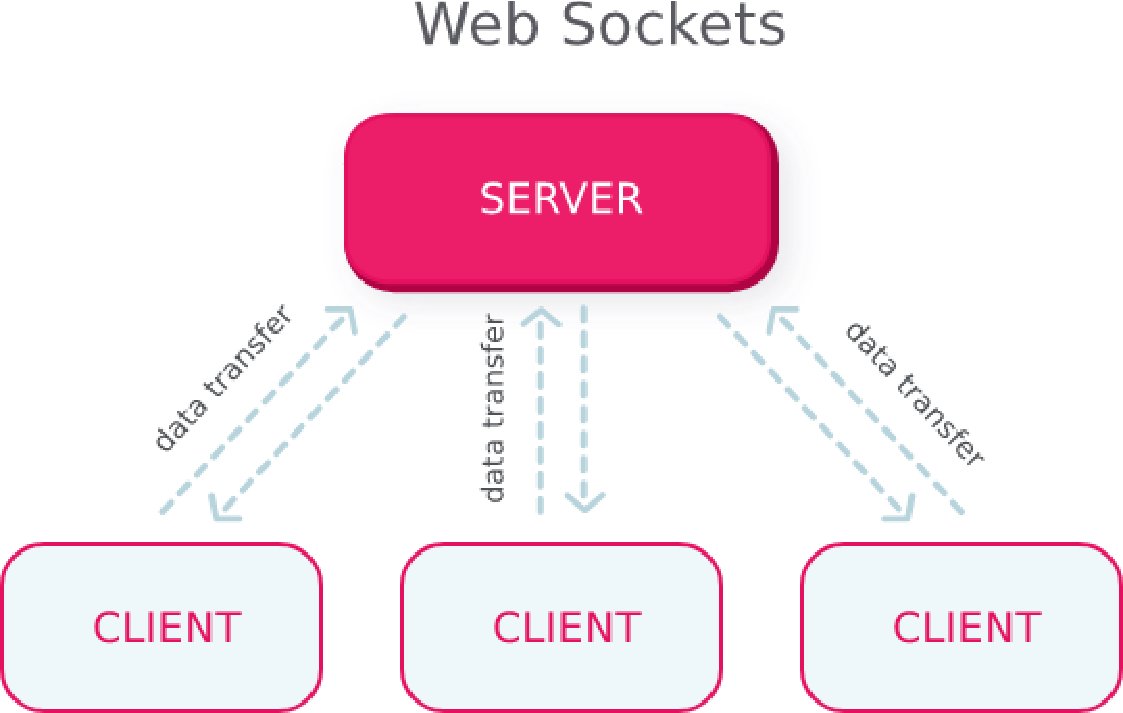
\includegraphics[width=.70\textwidth,angle=0]{figure 3-9.pdf}
    \caption{Štandardný režim fungovania webových soketov.}
    \captionsetup{font=footnotesize, justification=centering, skip=5pt}
    \caption*{(Zdroj: vlastné spracovanie)}
    \label{o:3-9}
\end{figure}  

\subsubsection{Architektúra}
Typická architektúra komunikačného systému dronu založeného na webových zásuvkách pozostáva z troch hlavných komponentov: pozemnej stanice, dronu a web-socket servera. Pozemná stanica je zodpovedná za generovanie používateľských príkazov a prijímanie telemetrických údajov a video prúdov z dronu. Dron je zodpovedný za vykonávanie príkazov a zachytávanie telemetrických údajov a video prúdov. Webový socketový server funguje ako middleware medzi pozemnou stanicou a dronom, spracováva komunikačný protokol a preposiela správy v reálnom čase (obrázok 3-9).



\subsubsection{Komunikačný protokol}
Komunikačný protokol pre systém dronu založený na webo-socket pozostáva z dvoch typov správ: príkazových správ a telemetrických správ.

\textbf{Príkazové správy.} Príkazové správy sa posielajú z pozemnej stanice do dronu a pozostávajú z pokynov pre dron, aby vykonal určitú činnosť, napríklad vzlietol, pristál, pohol sa dopredu alebo odbočil doľava. Formát príkazových správ sa môže líšiť v závislosti od modelu dronu a špecifických funkcií, ktoré sa používajú, ale bežný formát je JSON (JavaScript Object Notation). Napríklad príkazová správa o vzlete vo formáte JSON môže vyzerať takto:
\begin{verbatim}
{
  "command": "takeoff",
  "args": []
}
\end{verbatim}

\textbf{Telemetrické správy.} Príkazové správy sa posielajú z pozemnej stanice do dronu a pozostávajú z pokynov pre dron, aby vykonal určitú činnosť, napríklad vzlietol, pristál, pohol sa dopredu alebo odbočil doľava. Formát príkazových správ sa môže líšiť v závislosti od modelu dronu a špecifických funkcií, ktoré sa pTelemetrické správy sa odosielajú z dronu do pozemnej stanice a pozostávajú z údajov snímačov, ako sú súradnice GPS, nadmorská výška, úroveň nabitia batérie a údaje z kamery. Formát telemetrických správ sa môže líšiť aj v závislosti od modelu dronu a konkrétnych použitých snímačov, ale JSON je opäť bežný formát. Napríklad telemetrická správa Tello drona o svojom $state$ vo formáte JSON môže vyzerať takto:
\begin{verbatim}
    {
        "pitch": 0,
        "roll": 0,
        "yaw": 0,
        "vgx": 0,
        "vgy": 0,
        "vgz": 0,
        "templ": 62,
        "temph": 65,
        "tof": 10,
        "h": 0,
        "bat": 58,
        "baro": 40.39,
        "time": 0,
        "agx": 7.00,
        "agy": 19.00,
        "agz": -999.00
      }
\end{verbatim}
Tento objekt obsahuje rôzne informácie o stave dronu vrátane uhlov náklonu, natočenia a vychýlenia, rýchlosti pozdĺž osí x, y a z, teploty, vzdialenosti počas letu, úrovne nabitia batérie, barometrického tlaku a zrýchlenia pozdĺž osí x, y a z.

\subsubsection{Implementácia}
Na implementáciu komunikačného systému dronu založeného na web-sockets možno postupovať podľa nasledujúcich krokov:
\begin{itemize}
    \item Nastaviť web-socket server, ktorý dokáže spracovať prichádzajúce spojenia z pozemnej stanice a dronu a preposielať správy medzi nimi.
    \item Implementovať skript na strane klienta na pozemnej stanici, ktorý dokáže nadviazať spojenie webového socketu so serverom, odosielať príkazové správy do dronu a prijímať telemetrické správy z dronu.
    \item Implementovať skript na strane servera na dron, ktorý môže vytvoriť spojenie webového socketu so serverom, prijímať príkazové správy z pozemnej stanice a posielať telemetrické správy pozemnej stanici.
    \item Integrovať skripty na strane klienta a servera s riadiacim softvérom dronu a používateľským rozhraním na pozemnej stanici.
\end{itemize}
